\documentclass[class=scrartcl, crop=false]{standalone}
\usepackage[
typ={ohne},
fach=Informatik,
lerngruppe=SG-J1,
%loesungen=seite,
%lizenz={cc-by-nc-sa-4}
module={Aufgaben},
farbig
]{schule}
%\usepackage{polyglossia}
%\setmainlanguage{ngerman}
\usepackage[subpreambles=true]{standalone}
\usepackage{import}
\usepackage{fourier-otf}
\setmonofont{Ubuntu Mono Regular}[Scale=0.9]
\usepackage{shellesc}
\ShellEscape{pythontex \jobname.pytxcode }
\usepackage[
%prettyprinter=pygments, %pygopt={style=emacs}
]{pythontex}


\usepackage{hyperref}


\usepackage{booktabs}

\usepackage{minted}





\newcommand{\expandpyconc}[1]{\expandafter\reallyexpandpyconc\expandafter{#1}}
\newcommand{\reallyexpandpyconc}[1]{\pyconc{exec(compile(open('#1', 'rb').read(), '#1', 'exec'))}}

\newenvironment{pyconcodeblck}[1]
{\newcommand{\snippetfile}{snippet-#1.py}
	\VerbatimEnvironment
	\begin{VerbatimOut}{\snippetfile}}
	{\end{VerbatimOut}
	\expandpyconc{\snippetfile}}

\newcommand{\typesetcode}[1]{\inputpygments{python}{snippet-#1.py}}



\begin{document}

\section{Ein- und Ausgabe}
\begin{aufgabe} \noindent 
	Schreibe eine Funktion \mintinline{python}{greet_io}. Die Funktion fragt einen Benutzer nach seinem Namen und begrüßt diesen dann freundlich an der Konsole.
	\begin{figure}[H]
		\centering
		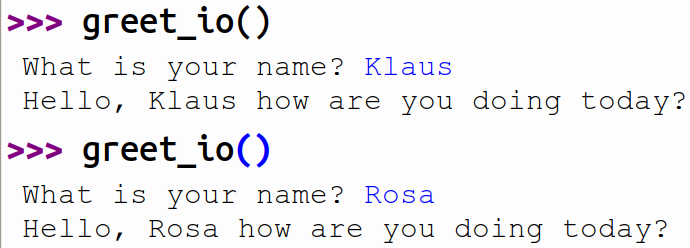
\includegraphics[width=0.6\linewidth]{greet_io}
		
		\label{fig:greet_io}
	\end{figure}
\end{aufgabe}




\begin{aufgabe} \noindent 
Schreibe eine Funktion \mintinline{python}{square_io}. Diese bittet den Benutzer eine Zahl einzugeben und gibt anschließend das Quadrat dieser Zahl an der Konsole aus.
% TODO: \usepackage{graphicx} required
\begin{figure}[H]
	\centering
	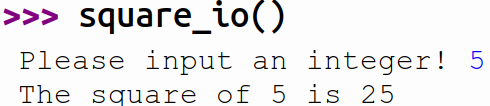
\includegraphics[width=0.6\linewidth]{square_io}

	\label{fig:square_io}
\end{figure}

\end{aufgabe}
\begin{aufgabe} \noindent 
	Schreibe eine Funktion \mintinline{python}{other_angle}. Diese bittet den Benutzer die Größen von zwei Winkel in einem Dreieck einzugeben und gibt anschließend die Größe des dritten Winkels an der Konsole aus.
	% TODO: \usepackage{graphicx} required
	\begin{figure}[H]
		\centering
		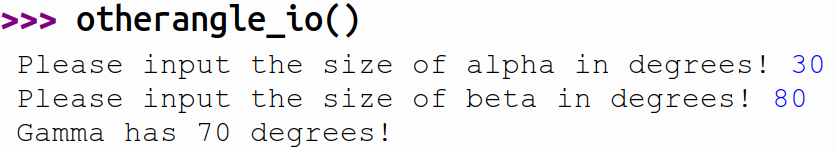
\includegraphics[width=0.6\linewidth]{other_angle_io}
		
		\label{fig:square_io}
	\end{figure}



\end{aufgabe}

\begin{aufgabe}
Untersuche deine Lösungen auf Codewiederholung und schreibe gegebenenfalls Hilfsfunktionen um diese zu vermeiden. Versuche außerdem so viel Code wie möglich in testbare Funktionen auszulagern.
\end{aufgabe}


\end{document}
